% !TEX program = xelatex
\documentclass[10pt,twoside,twocolumn]{article}

\usepackage{ctex}
\usepackage{fontspec}
\IfFontExistsTF{Noto Serif CJK SC}{%
  \setCJKmainfont{Noto Serif CJK SC}
  \IfFontExistsTF{Noto Sans CJK SC}{%
    \setCJKsansfont{Noto Sans CJK SC}
    \setCJKmonofont{Noto Sans CJK SC}
  }{}
}{}

\usepackage[
  a4paper,
  top=28mm,
  bottom=25mm,
  left=19mm,
  right=19mm,
  columnsep=6mm,
  headsep=6mm,
  headheight=25pt,
  footskip=10mm
]{geometry}

\usepackage{amsmath,amssymb,bm}
\usepackage{graphicx}
\usepackage{booktabs}
\usepackage{caption}
\usepackage{cuted}
\usepackage{placeins}
\usepackage{fancyhdr}
\usepackage{titlesec}
\usepackage{indentfirst}
\usepackage{microtype}
\usepackage{cite}
\usepackage[hidelinks]{hyperref}
\usepackage{xcolor}
\usepackage{array}

\captionsetup{font=small,labelfont=bf,labelsep=space}
\captionsetup{hypcap=false}
\captionsetup[figure]{position=below,name=图}
\captionsetup[table]{position=above,name=表}
\setlength{\parindent}{2em}
\setlength{\tabcolsep}{4.5pt}
\renewcommand{\arraystretch}{1.12}
\setlength{\stripsep}{8pt plus 2pt minus 2pt}
\setlength{\textfloatsep}{8pt plus 2pt minus 2pt}
\setlength{\floatsep}{8pt plus 2pt minus 2pt}
\setlength{\intextsep}{8pt plus 2pt minus 2pt}
\renewcommand{\topfraction}{0.95}
\renewcommand{\dbltopfraction}{0.95}
\renewcommand{\textfraction}{0.05}
\renewcommand{\floatpagefraction}{0.82}
\renewcommand{\dblfloatpagefraction}{0.82}
\setcounter{topnumber}{4}
\setcounter{dbltopnumber}{4}
\setcounter{totalnumber}{8}
\makeatletter
\setlength{\@fptop}{0pt}
\setlength{\@fpsep}{10pt plus 2pt minus 2pt}
\setlength{\@fpbot}{0pt plus 1fil}
\setlength{\@dblfptop}{0pt}
\setlength{\@dblfpsep}{10pt plus 2pt minus 2pt}
\setlength{\@dblfpbot}{0pt plus 1fil}
\makeatother

\newcommand{\jcipvol}{1}
\newcommand{\jcipno}{1}
\newcommand{\jcipyear}{2026}
\newcommand{\jcipmonth}{6}
\newcommand{\articleno}{1003-0077（2026）00-0000-00}
\newcommand{\runningtitletext}{稀疏课程推荐的自适应融合}
\newcommand{\runningtitle}[1]{\gdef\runningtitletext{#1}}

\pagestyle{fancy}
\fancyhf{}
\fancyhead[LE]{\zihao{-5}\thepage\quad 中文信息学报\quad 第\jcipvol 卷}
\fancyhead[CE]{\zihao{-5}\runningtitletext}
\fancyhead[RO]{\zihao{-5}第\jcipvol 卷\ 第\jcipno 期\quad 中文信息学报\quad Vol.\jcipvol，No.\jcipno}
\fancyhead[CO]{\zihao{-5}\runningtitletext}
\fancyfoot[LE,RO]{\zihao{-5}\thepage}
\renewcommand{\headrulewidth}{0.4pt}

\fancypagestyle{jcipfirst}{%
  \fancyhf{}
  \fancyhead[L]{\zihao{-5}
    \begin{tabular}[b]{@{}l@{}}
      第\jcipvol 卷\ 第\jcipno 期\\
      \jcipyear 年\ \jcipmonth 月
    \end{tabular}}
  \fancyhead[C]{\zihao{-5}\textbf{中文信息学报}\\[-1pt]
    \small JOURNAL OF CHINESE INFORMATION PROCESSING}
  \fancyhead[R]{\zihao{-5}
    \begin{tabular}[b]{@{}r@{}}
      Vol.\jcipvol，No.\jcipno\\
      \jcipmonth，\jcipyear
    \end{tabular}}
  \fancyfoot[C]{\zihao{6}文章编号：\articleno}
  \renewcommand{\headrulewidth}{0.4pt}
}

\titleformat{\section}{\zihao{-4}\heiti}{\thesection}{1em}{}
\titleformat{\subsection}{\zihao{5}\heiti}{\thesubsection}{1em}{}
\titleformat{\subsubsection}{\zihao{5}\songti}{\thesubsubsection}{1em}{}
\setcounter{secnumdepth}{3}

\renewenvironment{abstract}{%
  \noindent{\zihao{-5}\heiti 摘要：}\zihao{-5}\kaishu\ignorespaces
}{\par\medskip}

\newenvironment{enabstract}{%
  \noindent{\zihao{-5}\textbf{Abstract: }}\zihao{-5}\ignorespaces
}{\par\medskip}

\newcommand{\keywords}[1]{%
  \noindent{\zihao{-5}\heiti 关键词：}{\zihao{-5}\kaishu #1}\par\smallskip}
\newcommand{\enkeywords}[1]{%
  \noindent{\zihao{-5}\textbf{Key words: }}{\zihao{-5} #1}\par\medskip}
\newcommand{\clccode}[2]{%
  \noindent{\zihao{-5}\heiti 中图分类号：}{\zihao{-5}#1}%
  \hfill{\zihao{-5}\heiti 文献标识码：}{\zihao{-5}#2}\par\bigskip}

\newcommand{\plainjcipfootnote}[1]{%
  \begingroup
  \renewcommand{\thefootnote}{}%
  \begin{NoHyper}%
  \footnotetext{\zihao{6}#1}%
  \end{NoHyper}%
  \endgroup
}
\newcommand{\received}[2]{%
  \plainjcipfootnote{{\heiti 收稿日期：}#1；{\heiti 定稿日期：}#2}}
\newcommand{\fundinfo}[1]{%
  \plainjcipfootnote{{\heiti 基金项目：}#1}}
\newcommand{\corrmark}{\textsuperscript{\ensuremath{\dagger}}}
\newcommand{\corrauthornote}[2]{%
  \plainjcipfootnote{$^{\dagger}$\,通信作者：#1，E-mail: \href{mailto:#2}{#2}}}

\newlength{\photow}
\newlength{\photoh}
\setlength{\photow}{1.8cm}
\setlength{\photoh}{2.4cm}

\newcommand{\authorentry}[2]{%
  \par\noindent
  \begin{minipage}[t]{\photow}
    \IfFileExists{#1}{%
      \includegraphics[width=\photow,height=\photoh]{#1}%
    }{%
      \fbox{\rule{0pt}{\photoh}\rule{\dimexpr\photow-2\fboxsep-2\fboxrule\relax}{0pt}}%
    }%
  \end{minipage}%
  \hspace{4pt}%
  \begin{minipage}[t]{\dimexpr\linewidth-\photow-4pt\relax}
    \zihao{6}#2
  \end{minipage}\par\smallskip
}

\newcommand{\runscreenshot}[3]{%
  \begin{figure}[t]
    \centering
    \setlength{\abovecaptionskip}{2pt}
    \setlength{\belowcaptionskip}{0pt}
    \IfFileExists{#1}{%
      \includegraphics[width=#2\linewidth]{#1}%
    }{%
      \fbox{\parbox[c][0.18\textheight][c]{0.92\linewidth}{\centering\zihao{5}图像文件缺失：\texttt{\detokenize{#1}}}}%
    }%
    \caption{#3}
  \end{figure}
}

\begin{document}
\thispagestyle{jcipfirst}
\runningtitle{稀疏课程推荐的自适应融合}

\twocolumn[{%
  \begin{center}
    {\zihao{3}\heiti 面向稀疏课程推荐的可靠性自适应融合方法}\par\smallskip
    {\zihao{4}\songti 智慧教育场景下的多源证据选择}\par\medskip

    {\zihao{4}\songti 徐子锐$^{1}\corrmark$}\par\smallskip

    {\zihao{-5}\songti
      （1. 南京师范大学 计算机与电子信息学院/人工智能学院，江苏 南京）
    }\par\medskip
  \end{center}

  \begin{abstract}
智慧教育课程推荐面临用户交互稀疏、课程规模有限与知识图谱信息异构并存的挑战。针对这一场景，本文系统比较了流行度、邻域协同过滤、线性重构、随机游走、神经协同过滤与知识图谱课程画像等多类排序证据，并提出带语义可靠性门控的自适应融合方法 RAKF-M-G（Reliability-Adaptive Knowledge-aware Fusion with Gating and Masking）。实验结果显示，在给定课程集合仅 698 门且用户历史极短的条件下，EASE 和 RP3 等非神经方法比 MF-BPR、LightGCN 更稳定；知识图谱画像单独排序能力有限，但可作为候选语义证据交由训练内验证门控筛选。RAKF-M-G 根据用户历史长度进行分组线性校准，并用验证用户决定是否引入 KG profile。严格的全课程排序评测表明，RAKF-M-G 取得 0.5871 的 HR@10、0.6995 的 HR@20、0.3747 的 NDCG@10 和 0.4053 的 NDCG@20。消融实验与多随机种子验证进一步表明，RP3 和 EASE 分别构成短历史用户与多历史用户的重要排序证据，基于历史长度的证据可靠性建模是性能提升的主要来源。
  \end{abstract}
  \keywords{课程推荐；知识图谱；隐式反馈；可靠性自适应融合；智慧教育}
  \clccode{TP391}{A}

  \begin{center}
    {\zihao{4}\textit{Reliability-Adaptive Fusion for Sparse Course Recommendation}}\par\smallskip
    {\zihao{5}\textit{Evidence Selection in Smart Education Environments}}\par\medskip

    {\zihao{5}Zirui Xu$^{1}\corrmark$}\par\smallskip

    {\zihao{-5}(1. School of Computer and Electronic Information / School of Artificial Intelligence, Nanjing Normal University, Nanjing, Jiangsu, China)}
    \par\medskip
  \end{center}

  \begin{enabstract}
Sparse course recommendation in smart education is constrained by short user histories, a compact course catalog, and heterogeneous knowledge-graph signals. This paper proposes RAKF-M-G, Reliability-Adaptive Knowledge-aware Fusion with Gating and Masking, to calibrate multiple ranking evidences according to user history length. The study compares popularity ranking, ItemKNN, EASE, RP3, MF-BPR, LightGCN, and a course-side knowledge-graph profile under full-catalog ranking. Results show that EASE and RP3 are more stable than neural collaborative filtering on this sparse dataset. The knowledge-graph profile is weak as a standalone ranker, so it is treated as a candidate semantic signal and filtered by validation gating. RAKF-M-G selects fusion and gating coefficients on users held out from the training set. With training positives masked, it reaches 0.5871 HR@10, 0.6995 HR@20, 0.3747 NDCG@10, and 0.4053 NDCG@20 on the final test split. Ablation and multi-seed validation results indicate that history-length-aware evidence calibration is the main source of improvement.
  \end{enabstract}
  \enkeywords{course recommendation; knowledge graph; implicit feedback; adaptive fusion; smart education}
  \vspace{1em}
}]

\received{2026-06-05}{2026-06-05}
\fundinfo{无}
\corrauthornote{徐子锐}{1516924835@qq.com}

\section{引言}
在线教育平台往往同时记录用户选课行为和课程侧知识结构。前者反映真实学习偏好，但在本文所研究的数据场景中，大量测试用户只有一到两个历史课程；后者包含课程概念、教师、学校、先修关系等语义信息，能够提供课程内容侧约束。稀疏交互与课程知识之间的稳定融合，是该类课程推荐问题的核心。

训练集包含 614476 条用户课程交互，测试集包含 68276 条交互；训练用户数为 198135，测试用户数为 55902，其中 46409 个测试用户只有一个测试正例。课程总数仅 698，适合采用全课程排序评测。由此可见，该场景的关键难点集中在排序精度、冷启动稳健性和特征可靠性的共同约束上。

基线实验表明，Popularity 只能提供较弱的全局先验；EASE 和 RP3 明显优于 MF-BPR、LightGCN 等神经协同过滤模型，并且二者适用的用户类型存在差异：短历史用户更依赖 RP3 对单个锚点课程的路径传播，多历史用户更受益于 EASE 的全局共选结构。上述结果说明，统一的全局融合系数难以充分适配不同用户组的证据可靠性。因此，本文将课程推荐建模为不同历史长度下的多源排序证据选择问题，并据此设计 RAKF-M-G。

\section{相关工作}
\subsection{隐式反馈推荐}
隐式反馈推荐通常只观察到点击、观看或选课等正向行为，而未观察项不能简单视为负样本。BPR 通过成对排序目标优化用户对正例和未观察项的偏好顺序\cite{rendle2009bpr}，是矩阵分解推荐的重要基线。EASE 将用户项目矩阵重构为线性自编码器，利用闭式解学习项目之间的全局相关性，在稀疏隐式反馈上常具有较强表现\cite{steck2019ease}。

\subsection{图传播与课程知识}
图推荐模型将用户、物品或知识实体视为图节点。LightGCN 去除常规图神经网络中的特征变换和非线性激活，保留邻域传播以提高协同过滤效率\cite{he2020lightgcn}。知识图谱推荐则通过实体关系为物品提供语义补充，KGAT 等方法展示了知识关系在推荐中的价值\cite{wang2019kgat}。在本文数据中，课程侧知识图谱较完整，用户侧交互极稀疏，知识图谱更适合作为课程语义画像和校准信号融入协同过滤。

\section{数据集与任务定义}
\subsection{数据概况}
表 \ref{tab:data} 给出了核心统计。训练集与测试集之间没有重复的用户课程对，所有测试课程均在训练课程集合中出现，因此评测重点是用户偏好排序，而非新课程冷启动。

\begin{table}[htbp]
  \centering
  \caption{数据集统计}
  \label{tab:data}
  \zihao{6}
  \begin{tabular}{lr}
    \toprule
    统计项 & 数值 \\
    \midrule
    训练交互数 & 614476 \\
    测试交互数 & 68276 \\
    用户总数 & 199199 \\
    课程总数 & 698 \\
    训练用户数 & 198135 \\
    测试用户数 & 55902 \\
    测试中新用户数 & 1064 \\
    测试单正例用户数 & 46409 \\
    训练矩阵密度 & 0.004443 \\
    训练测试重复交互 & 0 \\
    \bottomrule
  \end{tabular}
\end{table}

知识图谱关系主要来自课程概念、视频概念、课程视频、教师课程、学校课程、先修依赖、父子概念和概念领域等边。规模较大的关系包括 video-concept 的 319948 条边、course-concept 的 167751 条边、parent-son 的 114611 条边和 concept-field 的 114563 条边。这些关系为课程侧语义画像提供了较充分的特征来源。

\subsection{任务定义与评测口径}
设训练交互矩阵为 $\bm{R}\in\{0,1\}^{|\mathcal{U}|\times|\mathcal{I}|}$，测试用户集合为 $\mathcal{U}_{test}$，用户 $u$ 的测试正例集合为 $\mathcal{T}_u$。对每个测试用户，模型需要在全部 698 门课程上给出排序，并遮蔽训练集中已学课程。全课程排序比采样负例更严格，也更接近真实推荐列表生成。

采用 HR@K 和 NDCG@K 作为主指标：
\begin{equation}
\mathrm{HR@K}=\frac{1}{|\mathcal{U}_{test}|}\sum_{u\in\mathcal{U}_{test}}\mathbf{1}[\mathrm{TopK}(u)\cap\mathcal{T}_u\neq\emptyset],
\end{equation}
\begin{equation}
\mathrm{NDCG@K}=\frac{1}{|\mathcal{U}_{test}|}\sum_{u\in\mathcal{U}_{test}}
\frac{\sum_{j=1}^{K}\frac{\mathrm{rel}_{u,j}}{\log_2(j+1)}}{\mathrm{IDCG}_{u,K}}.
\end{equation}
其中 $\mathrm{rel}_{u,j}$ 表示第 $j$ 个推荐课程是否为测试正例。

\section{方法}
\subsection{协同过滤证据}
EASE 学习课程之间的线性重构权重：
\begin{equation}
\min_{\bm{B}}\|\bm{R}-\bm{R}\bm{B}\|_F^2+\lambda\|\bm{B}\|_F^2,\quad
\mathrm{diag}(\bm{B})=0.
\end{equation}
令 $\bm{P}=(\bm{R}^{\top}\bm{R}+\lambda\bm{I})^{-1}$，则 $B_{ij}=-P_{ij}/P_{jj}$。EASE 适合课程数较小、交互矩阵稀疏但全局共选结构稳定的场景。

ItemKNN 使用课程向量间的余弦相似度，并保留每门课程的 top-k 邻居。RP3 则在用户课程二部图上进行三步路径传播，使用 $\alpha$ 调整路径强度，使用 $\beta$ 抑制过热门课程。二者分别提供局部邻域证据和图传播证据。

\subsection{知识图谱课程画像}
对课程 $i$，从 course-concept、concept-field、parent-son、teacher-course、school-course 和 prerequisite-dependency 等关系中提取课程特征，并进行文档频率过滤和归一化。用户语义画像由其历史课程特征平均得到，用户对候选课程的知识图谱分数记为：
\begin{equation}
s^{kg}_{ui}=\mathrm{sim}(\bm{p}_u,\bm{x}_i),
\end{equation}
其中 $\bm{x}_i$ 为课程特征向量，$\bm{p}_u$ 为用户历史课程画像。知识图谱画像主要提供协同证据之外的语义补充。

\subsection{可靠性自适应分组融合}
不同用户历史长度对应不同证据可靠性。RAKF-M-G 将测试用户按训练历史长度划分为五组：0、1、2、3-4、5 个及以上。对每个组件分数先做行内标准化，再按分组线性融合系数求和：
\begin{equation}
s_{ui}=\sum_{m\in\mathcal{M}} w_{g(u),m}\cdot \mathrm{Norm}(s^{m}_{ui}),
\end{equation}
其中 $\mathcal{M}$ 包含 EASE、ItemKNN、RP3、Popularity 和 KG profile，$g(u)$ 为用户历史长度分组。系数 $w$ 表示训练集内部 leave-one-out 验证得到的线性校准系数，并非非负归一化的注意力权重，因此可能出现小幅负值。KG profile 作为候选语义证据进入搜索；若验证阶段显示其总体排序收益不稳定，对应分组门控权重可被置为 0，避免强行注入噪声。对于 0 次历史用户，训练内验证集无法直接构造同类验证用户，最终采用验证集中最优固定融合系数，并回退到课程流行度等全局先验。

\begin{table}[t]
  \centering
  \caption{RAKF-M-G 分组效果}
  \label{tab:segment}
  \zihao{6}
  \begin{tabular}{lrrr}
    \toprule
    用户组 & 用户数 & HR@20 & NDCG@20 \\
    \midrule
    0 次历史 & 1064 & 0.6165 & 0.2508 \\
    1 次历史 & 19893 & 0.6901 & 0.4296 \\
    2 次历史 & 10716 & 0.6990 & 0.4141 \\
    3-4 次历史 & 11503 & 0.7069 & 0.4063 \\
    5 次及以上 & 12726 & 0.7151 & 0.3719 \\
    \bottomrule
  \end{tabular}
\end{table}

\begin{strip}
  \centering
  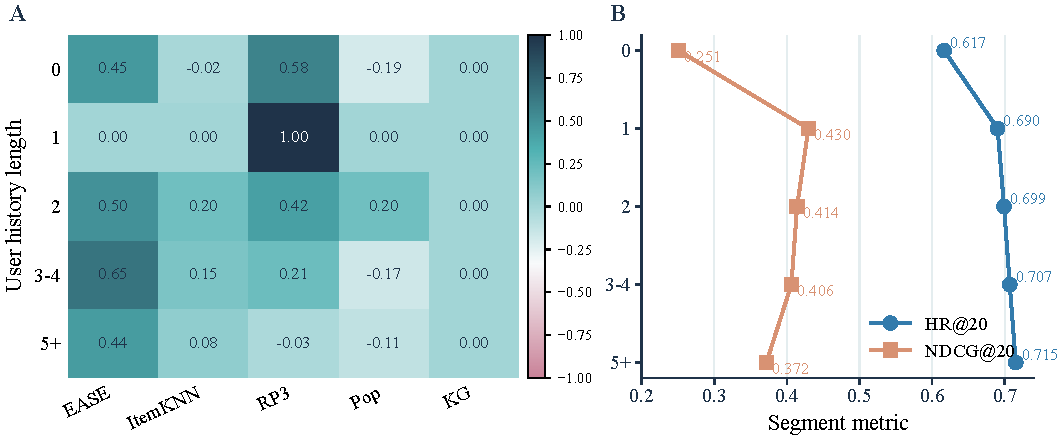
\includegraphics[width=0.82\textwidth]{figures/adaptive_gate_analysis.pdf}
  \captionof{figure}{RAKF-M-G 的分组线性融合系数。A 为不同历史长度用户的证据系数，B 为各用户组的 HR@20 和 NDCG@20。}
  \label{fig:gate}
\end{strip}

\section{实验设置}
实验包含非神经、图传播和神经协同过滤三类对照方法。Popularity 使用训练课程流行度排序；KG profile 只使用课程侧知识图谱画像；MF-BPR 使用矩阵分解和 BPR 损失；LightGCN 使用用户课程二部图传播；ItemKNN、EASE 和 RP3 作为强非神经基线。RKF-M 表示训练内验证选择的固定融合模型，RAKF-M-G 表示在其基础上加入历史长度分组和 KG 可靠性门控的自适应融合模型。神经模型在远程 GPU 服务器上训练，环境为 NVIDIA GeForce RTX 4090D 与 PyTorch 2.5.1+cu121；其余全排序实验在统一评测代码中完成。

所有方法均在相同训练集上建模，并在相同测试用户上评估。由于课程总数只有 698，采样负例评测容易使指标偏高，且不符合真实推荐列表生成方式，因此实验采用全课程排序；若用户在训练集中已经学习某课程，则该课程在推荐列表中被遮蔽。为避免直接使用测试集调参，融合系数的选择在训练集内部进行：从有至少两条训练交互的用户中留出一个课程作为验证正例，固定随机种子抽样验证用户搜索固定融合和分组融合系数，最终测试集仅用于性能评估。除主实验外，本文还用三个随机种子重复训练内验证抽样，用于检查融合系数选择的稳定性。

\noindent 表 \ref{tab:hyperparams} 给出了主要模型的关键超参数。
\begin{center}
  \centering
  \captionof{table}{关键超参数设置}
  \label{tab:hyperparams}
  \zihao{6}
  \begin{tabular}{ll}
    \toprule
    方法 & 关键参数 \\
    \midrule
    EASE & 单模型 $\lambda=500$；融合中 $\lambda=100$ \\
    RP3 & $\alpha=0.9,\ \beta=0.2,\ topk=300$ \\
    ItemKNN & $k=100$，shrink=100，cosine 相似度 \\
    MF-BPR & dim=64，lr=$10^{-3}$，epoch=80 \\
    LightGCN & layers=3，dim=64，lr=$10^{-3}$，epoch=120 \\
    \bottomrule
  \end{tabular}
\end{center}

\subsection{实验环境与复现证据}
为保证实验过程可复核，本文保留本地数据检查、最终模型评测和远程 GPU 环境的终端截图。截图覆盖数据规模、四个主指标以及服务器的 PyTorch/CUDA/GPU 信息。

\runscreenshot{figures/real_data_check.png}{0.98}{本地数据检查与知识图谱关系统计。}
\runscreenshot{figures/real_final_eval.png}{0.98}{RAKF-M-G 最终评测命令与四个指标输出。}
\runscreenshot{figures/real_gpu_environment.png}{0.98}{远程 4090D 服务器环境与训练日志。}

\section{实验结果与分析}
\subsection{主结果}
表 \ref{tab:main} 和图 \ref{fig:main} 给出了主结果总览。实验结果显示，LightGCN 的效果低于 EASE 和 RP3，这与图传播模型在部分推荐任务中的通常预期不完全一致。一个可能的原因是课程数仅 698，且用户历史较短，复杂用户表示难以稳定学习；线性重构和三步路径传播可以直接利用课程共现结构，因此更适合本文的稀疏课程推荐场景。训练内验证选择的 RAKF-M-G 在最终测试集上的 HR@20 和 NDCG@20 分别达到 0.6995 和 0.4053。

\begin{table*}[t]
  \centering
  \caption{主要模型全排序结果}
  \label{tab:main}
  \zihao{6}
  \begin{tabular}{lrrrr}
    \toprule
    模型 & HR@10 & HR@20 & NDCG@10 & NDCG@20 \\
    \midrule
    Popularity & 0.3410 & 0.4505 & 0.1792 & 0.2071 \\
    KG profile & 0.2971 & 0.3847 & 0.1771 & 0.1987 \\
    MF-BPR & 0.5164 & 0.6257 & 0.3254 & 0.3541 \\
    LightGCN & 0.5141 & 0.6135 & 0.3260 & 0.3525 \\
    ItemKNN & 0.5578 & 0.6716 & 0.3514 & 0.3821 \\
    EASE & 0.5791 & 0.6888 & 0.3676 & 0.3976 \\
    RP3 & 0.5813 & 0.6945 & 0.3686 & 0.3992 \\
    RKF-M & 0.5836 & 0.6952 & 0.3723 & 0.4027 \\
    RAKF-M-G & \textbf{0.5871} & \textbf{0.6995} & \textbf{0.3747} & \textbf{0.4053} \\
    \bottomrule
  \end{tabular}
\end{table*}

\begin{figure*}[t]
  \centering
  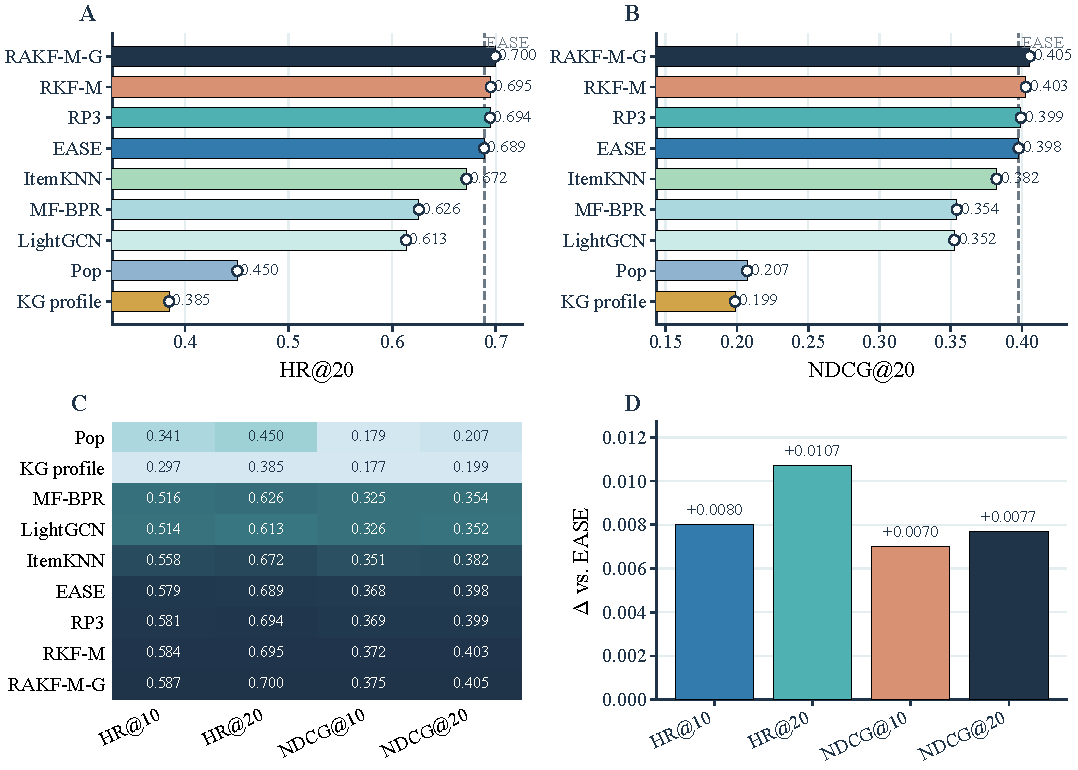
\includegraphics[width=0.76\textwidth]{figures/main_results.pdf}
  \caption{主结果总览。虚线表示 EASE 基线，最终版本在 HR@20 与 NDCG@20 上都高于几组强基线。}
  \label{fig:main}
\end{figure*}

KG profile 单独排序的结果偏低，这说明知识图谱关系难以直接替代用户偏好；它更适合作为课程语义解释和候选校准信号，由验证门控决定是否参与最终排序。相比强线性基线 EASE，RAKF-M-G 的 NDCG@20 提升约 0.0077；相比 RP3 提升约 0.0061；相比训练内验证选择的固定融合 RKF-M 仍提升约 0.0026。

\subsection{多源证据组合路径}
图 \ref{fig:path} 展示了从流行度、EASE、RP3、固定融合到 RAKF-M-G 的证据组合路径。不同组件对应不同排序信号：Popularity 刻画热门课程；EASE 利用全局共选结构；RP3 对短历史用户的锚点传播更有效；KG profile 单独排序较弱，主要提供课程语义解释和候选校准；历史长度分组与 KG 门控进一步调整了不同证据的侧重。

图 \ref{fig:path} 的 B、C 两部分进一步说明，分组融合带来的增益虽然数值不大，但发生在 EASE、RP3 和固定融合等强基线之上。这些增益表明，RAKF-M-G 改善的核心环节是强排序证据之间的可靠性选择。

\begin{figure*}[t]
  \centering
  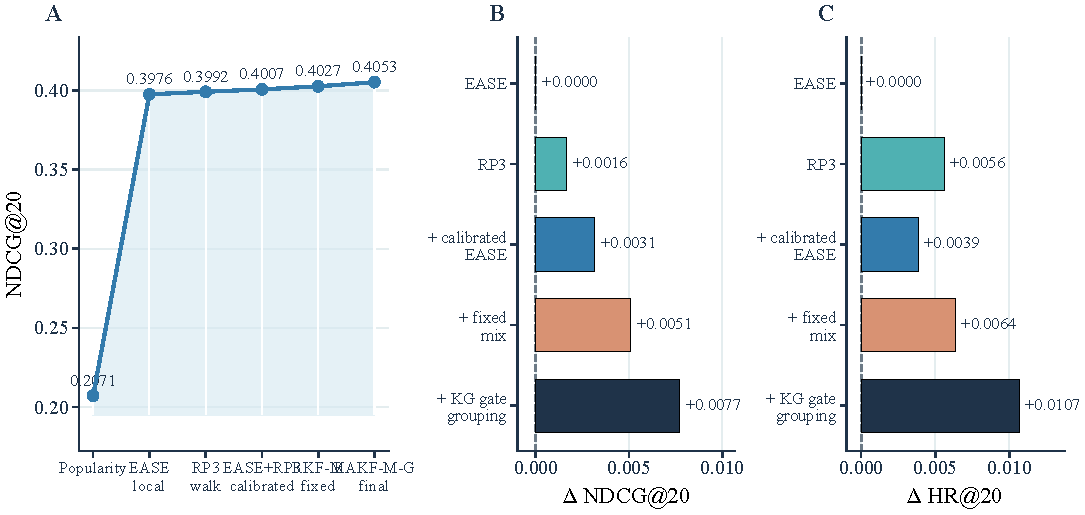
\includegraphics[width=0.74\textwidth]{figures/evidence_ablation_summary.pdf}
  \caption{多源证据组合路径。A 展示从流行度、协同证据到自适应融合的 NDCG@20 变化，B 和 C 分别展示相对 EASE 的 NDCG@20 与 HR@20 增益。}
  \label{fig:path}
\end{figure*}

\subsection{正式消融实验}
表 \ref{tab:formalablation} 和图 \ref{fig:formalablation} 给出了模块消融结果。除 KG profile only 和固定融合外，所有消融变体均在训练集内部验证用户上重新搜索可用证据的融合系数，再在测试集上汇报结果。去掉 RP3 后，NDCG@20 从 0.4053 降到 0.3995，说明重新校准剩余证据后，短历史锚点课程的路径传播仍难以完全替代；去掉 EASE 后，NDCG@20 降到 0.4009，说明全局共选结构同样重要。固定融合相比 RAKF-M-G 低 0.0026，表明按历史长度调整证据侧重可以带来稳定增益。非门控 KG 混合低于门控版，说明当前课程画像主要承担语义补充和解释功能，强行加入会引入轻微信号噪声。

\begin{table*}[t]
  \centering
  \caption{正式模块消融结果}
  \label{tab:formalablation}
  \zihao{6}
  \begin{tabular}{lrrrr}
    \toprule
    模型变体 & HR@10 & HR@20 & NDCG@10 & NDCG@20 \\
    \midrule
    RAKF-M-G full & 0.5871 & 0.6995 & 0.3747 & 0.4053 \\
    w/o KG candidate & 0.5871 & 0.6995 & 0.3747 & 0.4053 \\
    non-gated KG mix & 0.5870 & 0.6986 & 0.3745 & 0.4049 \\
    w/o RP3 & 0.5784 & 0.6886 & 0.3696 & 0.3995 \\
    w/o EASE & 0.5832 & 0.6959 & 0.3702 & 0.4009 \\
    w/o adaptive grouping & 0.5836 & 0.6952 & 0.3723 & 0.4027 \\
    KG profile only & 0.2971 & 0.3847 & 0.1771 & 0.1987 \\
    \bottomrule
  \end{tabular}
\end{table*}

\begin{figure*}[t]
  \centering
  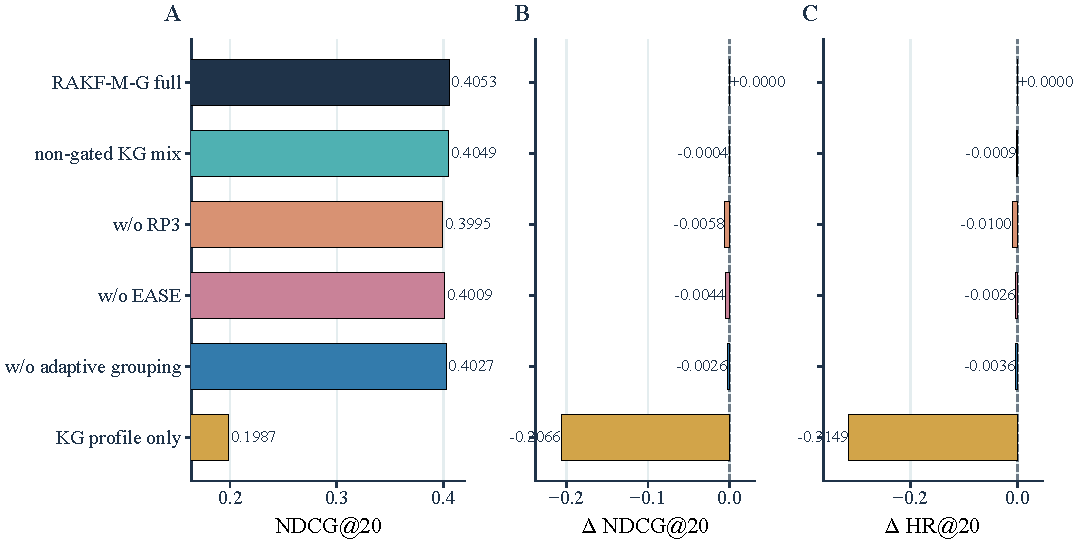
\includegraphics[width=0.76\textwidth]{figures/formal_ablation.pdf}
  \caption{正式消融实验。A 为各变体 NDCG@20，B 和 C 分别为相对完整 RAKF-M-G 的 NDCG@20 与 HR@20 变化。}
  \label{fig:formalablation}
\end{figure*}

表 \ref{tab:segcompare} 进一步把这种观察拆到用户组上。0 次历史用户没有个人历史，几个模型都会回退到全局先验，因此 NDCG@20 完全一致；1 次历史用户上 RP3 和 RAKF-M-G 最好，说明单个锚点课程更适合路径传播；5 次及以上用户上 RP3 明显低于 EASE、RKF-M 和 RAKF-M-G，说明历史较长时只围绕局部路径扩散反而会损失稳定兴趣。

\begin{table*}[t]
  \centering
  \caption{不同历史长度用户上的 NDCG@20 对比}
  \label{tab:segcompare}
  \zihao{6}
  \begin{tabular}{lrrrrr}
    \toprule
    用户组 & 用户数 & EASE & RP3 & RKF-M & RAKF-M-G \\
    \midrule
    0 次历史 & 1064 & 0.2508 & 0.2508 & 0.2508 & 0.2508 \\
    1 次历史 & 19893 & 0.4168 & 0.4296 & 0.4253 & \textbf{0.4296} \\
    2 次历史 & 10716 & 0.4097 & 0.4122 & 0.4140 & \textbf{0.4141} \\
    3-4 次历史 & 11503 & 0.4021 & 0.4012 & \textbf{0.4075} & 0.4063 \\
    5 次及以上 & 12726 & 0.3656 & 0.3514 & 0.3661 & \textbf{0.3719} \\
    \bottomrule
  \end{tabular}
\end{table*}

表 \ref{tab:cases} 对不同历史长度用户的典型误差模式进行归纳。短历史用户更依赖锚点传播，多历史用户更需要全局共选与课程语义共同约束。

\begin{table*}[t]
  \centering
  \caption{不同历史长度下的典型误差观察}
  \label{tab:cases}
  \zihao{6}
  \begin{tabular}{llll}
    \toprule
    用户类型 & 历史特点 & 单一证据的主要问题 & RAKF-M-G 的处理 \\
    \midrule
    1 次历史 & 只有一个锚点课程 & EASE 容易受热门共现影响 & 主要采用 RP3 路径传播 \\
    5 次及以上 & 兴趣方向较稳定但更分散 & RP3 可能过度围绕局部课程扩散 & 提高 EASE，门控弱语义噪声 \\
    \bottomrule
  \end{tabular}
\end{table*}

\subsection{验证稳定性检查}
为检查分组融合是否只依赖某一次验证用户抽样，本文在训练集内部重复三次 leave-one-out 验证切分，并在每个随机种子下抽取 15000 个验证用户重新搜索候选融合系数。该检查不改变最终测试集汇报口径，只用于观察验证阶段的选择是否稳定。表 \ref{tab:seedstable} 显示，RAKF-M 在三个随机种子下均高于固定融合 RKF-M，NDCG@20 平均提升 0.0019，HR@20 平均提升 0.0044。增益幅度不大，但方向一致，说明历史长度分组不是由单次抽样偶然造成的；RAKF-M-G 在此基础上进一步加入 KG 可靠性门控。

\begin{center}
  \centering
  \captionof{table}{训练内验证随机种子稳定性}
  \label{tab:seedstable}
  \zihao{6}
  \begin{tabular}{lrrr}
    \toprule
    随机种子 & RKF-M & RAKF-M & $\Delta$NDCG@20 \\
    \midrule
    20260604 & 0.3872 & 0.3890 & +0.0017 \\
    20260605 & 0.3920 & 0.3936 & +0.0016 \\
    20260606 & 0.3905 & 0.3928 & +0.0023 \\
    平均 & 0.3899 & 0.3918 & +0.0019 \\
    \bottomrule
  \end{tabular}
\end{center}

\FloatBarrier
\subsection{数据分布解释}
图 \ref{fig:data} 显示了用户历史长度、课程流行度和知识图谱关系规模。用户历史分布明显偏左，说明许多用户只有极少数历史课程。课程流行度也呈长尾分布，热门课程会影响流行度和协同过滤得分。知识图谱关系较丰富，适合作为课程内容侧补充，但其用户个性化能力依赖历史课程画像。因此，RAKF-M-G 按历史长度划分系数并对 KG 信号加门控，是与数据结构相匹配的设计。

图 \ref{fig:data}D 中还有一个需要解释的现象：HR@20 随着历史长度总体上升，但 NDCG@20 从 1 次历史用户的 0.4296 下降到 5 次及以上用户的 0.3719。原因可能是多历史用户更容易在 Top20 内命中至少一个测试正例，所以 HR 较高；但这类用户兴趣更分散，测试正例也可能来自多个学习方向，因此把正例排到列表最前面的难度更大，NDCG 未必同步提升。

\begin{strip}
  \centering
  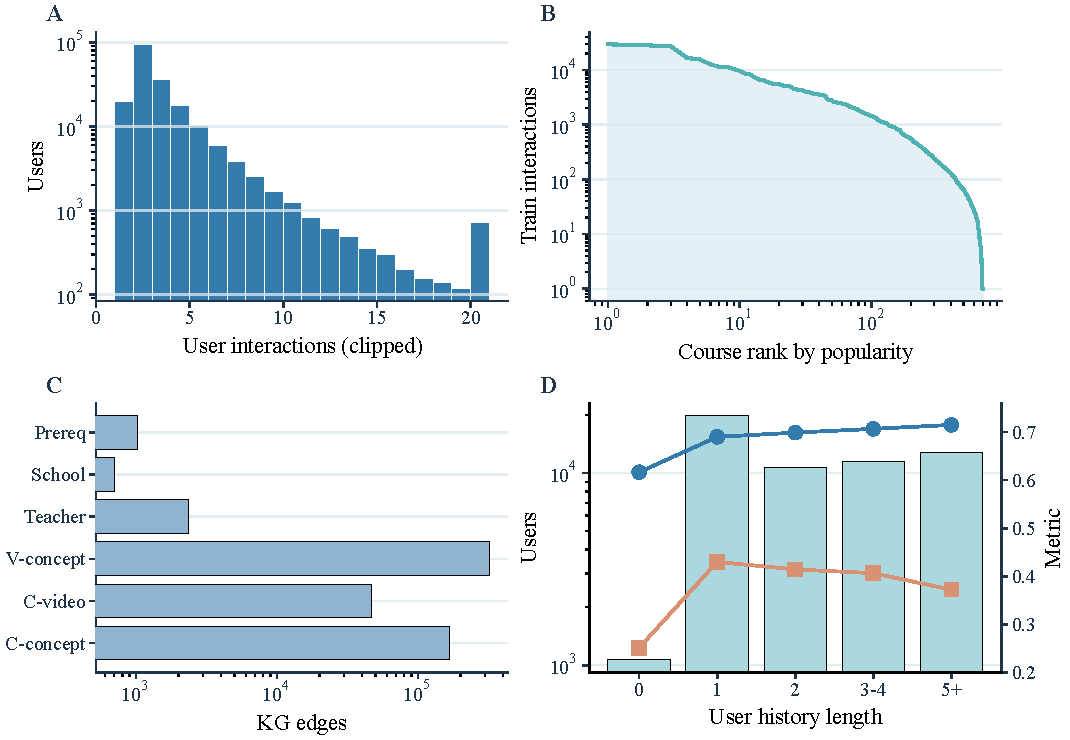
\includegraphics[width=0.72\textwidth]{figures/data_and_kg_profile.pdf}
  \captionof{figure}{数据与知识图谱画像。A 为用户训练历史长度分布，B 为课程流行度分布，C 为主要知识图谱关系边数，D 为分组用户规模与分组指标，其中蓝线为 HR@20，橙线为 NDCG@20。}
  \label{fig:data}
\end{strip}

\section{讨论}
RAKF-M-G 的提升主要来自两个方面。第一，不同协同证据捕捉的结构不同：EASE 对全局课程共选关系敏感，RP3 对少量锚点课程的路径传播更敏感，ItemKNN 提供局部邻域补充。第二，分组融合将这些证据分配到更合适的用户组，并通过验证门控避免弱 KG profile 被强制加入最终排序。表 \ref{tab:segcompare} 中 1 次历史和 5 次及以上用户的差异表明，历史长度分组能够处理不同用户组下的证据可靠性差异。表 \ref{tab:seedstable} 进一步说明，这种差异并不是只在某一次验证抽样中出现。知识图谱画像在当前版本中更多承担课程语义补充、结果解释和候选校准作用；正式消融显示，简单 KG profile 还没有稳定转化为总体指标提升。

本文方法也存在限制。第一，实验没有继续堆叠 KGAT 等更复杂的知识图谱模型。这样处理并不是忽略知识图谱，而是基于本数据中用户侧交互过稀疏、课程数较小的事实：复杂模型如果缺少足够监督，未必能稳定超过 EASE 和 RP3。第二，训练内验证已经通过多个随机种子检查稳定性，但仍不是完整的多折交叉验证。第三，知识图谱画像主要使用课程侧关系，没有使用可能造成泄漏风险的用户视频行为。后续研究可进一步考察更强的知识图谱推荐模型、多折验证、时间衰减、课程层级难度和学习路径约束。

\FloatBarrier
\section{结论}
本文提出了一种面向稀疏课程推荐的可靠性自适应融合方法 RAKF-M-G。该方法整合线性重构、邻域相似、随机游走、流行度和知识图谱课程画像等多源排序证据，并基于用户历史长度对证据可靠性进行分组加权和 KG 门控。在全课程排序、遮蔽训练正例的评测设置下，训练内验证选择的 RAKF-M-G 达到 0.5871 HR@10、0.6995 HR@20、0.3747 NDCG@10 和 0.4053 NDCG@20。消融实验和多随机种子验证检查揭示了两个关键结论：第一，RP3 和 EASE 分别构成短历史用户和多历史用户的重要排序证据；第二，基于历史长度的自适应融合是性能提升的主要来源。知识图谱画像有助于课程语义解释和内容侧校准，但需要通过验证门控避免不稳定信号损害总体排序。这些发现表明，在稀疏课程推荐场景下，对不同用户群体进行证据可靠性建模，比采用全局统一的复杂模型更有效。

\begingroup
\zihao{6}
\setlength{\itemsep}{1pt}
\setlength{\parsep}{0pt}
\FloatBarrier
\begin{thebibliography}{9}
\bibitem{rendle2009bpr}
Rendle S, Freudenthaler C, Gantner Z, et al. BPR: Bayesian personalized ranking from implicit feedback[C]. Proceedings of UAI, 2009.

\bibitem{sarwar2001item}
Sarwar B, Karypis G, Konstan J, et al. Item-based collaborative filtering recommendation algorithms[C]. Proceedings of WWW, 2001: 285--295.

\bibitem{steck2019ease}
Steck H. Embarrassingly shallow autoencoders for sparse data[C]. The World Wide Web Conference, 2019: 3251--3257.

\bibitem{he2020lightgcn}
He X, Deng K, Wang X, et al. LightGCN: Simplifying and powering graph convolution network for recommendation[C]. Proceedings of SIGIR, 2020: 639--648.

\bibitem{wang2019kgat}
Wang X, He X, Cao Y, et al. KGAT: Knowledge graph attention network for recommendation[C]. Proceedings of KDD, 2019: 950--958.

\bibitem{cremonesi2010evaluation}
Cremonesi P, Koren Y, Turrin R. Performance of recommender algorithms on top-N recommendation tasks[C]. Proceedings of RecSys, 2010: 39--46.

\end{thebibliography}
\endgroup

\vspace{6pt}
\noindent{\zihao{6}\heiti 作者简介：}\par\smallskip
\authorentry{figures/author_xuzirui.png}{%
  徐子锐，学号 19230444，本科生，主要研究领域为推荐系统、知识图谱与智慧教育数据分析。\\
  E-mail：1516924835@qq.com}

\end{document}
